\documentclass[12pt,fleqn]{article}\usepackage{../common}
\begin{document}
Ders 2

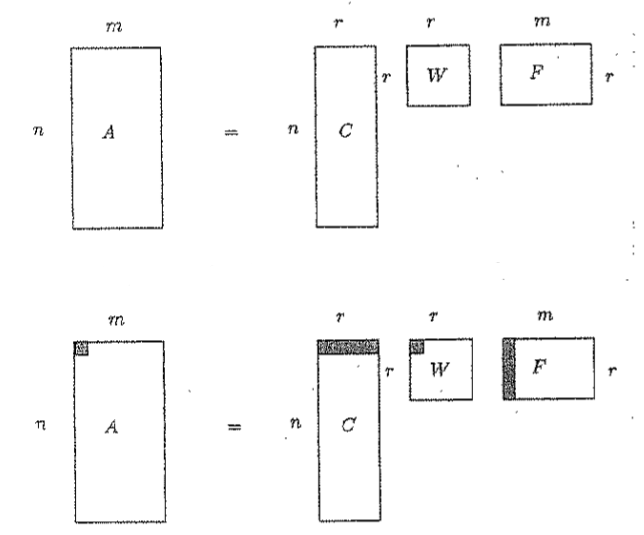
\includegraphics[height=7cm]{01.png}

Eger $r = 2$ olsa, $A$ icindeki herhangi bir 4 elemanli satir, $C$ uzerinde
onunla ayni sirada 2 elemanli baska bir satira tekabul edecekti, ve bu iki
elemanli satir $F$'deki ``faktorleri'' icindeki elemanlara gore agirlik
verecekti, yani carpip toplayacakti. 

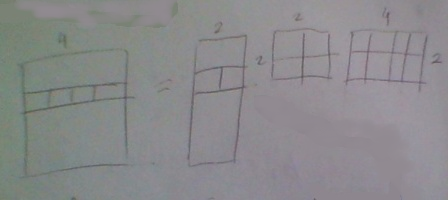
\includegraphics[height=4cm]{02.png}


\end{document}
